\documentclass[a4paper, 12pt]{article}
\usepackage[T1]{fontenc}
\usepackage{lmodern}
\usepackage{color}
\usepackage{amsfonts}
\usepackage{epstopdf}
\usepackage{matlab}
\usepackage{booktabs}
%\documentclass{book}
\usepackage{blindtext}
\usepackage{hyperref}
\usepackage[brazil]{babel}
\usepackage{amssymb}
\usepackage[utf8]{inputenc}
\usepackage{amsmath}
\usepackage{indentfirst}
\usepackage{graphicx}
\usepackage{listings}
\usepackage{tcolorbox}
\usepackage{upgreek}
\usepackage{multicol,lipsum}
\usepackage[a4paper,
top=3cm, left=3cm, bottom=3cm, right=3cm]{geometry}
\usepackage{setspace}
\usepackage{multirow}
\usepackage{float}
\usepackage[dvipsnames]{xcolor}
\usepackage[table]{xcolor}
%\usepackage{pdflscape}
\usepackage[DIV=15]{typearea}
\usepackage[nottoc]{tocbibind}
\usepackage[sort,numbers]{natbib}
%\usepackage{cite}
\usepackage{matlab}

\usepackage[utf8]{inputenc}
\usepackage[T1]{fontenc}
\usepackage{lmodern}
\usepackage{graphicx}
\usepackage{color}
\usepackage{hyperref}
\usepackage{amsmath}
\usepackage{amsfonts}
\usepackage{epstopdf}
\usepackage[table]{xcolor}
\usepackage{matlab}


\documentclass[letterpaper]{article}
% bib pack %%%%%%%%%%%%%%%%%%%%%%%%%%%%%%%%%%%%%%%%%%%%%%%%%%%%%%%%%%%%%%%%%%%%%
\usepackage[utf8]{inputenc}
\usepackage{geometry}
    \geometry{left=3cm,right=2cm,top=2cm,bottom=2cm}
%
\usepackage[spanish]{babel}
%
\usepackage[fixlanguage]{babelbib}
    \bibliographystyle{babunsrt}
%
\usepackage{url}

\begin{document}
%\maketitle

\begin{titlepage}
	\begin{center}
		

\vspace{10pt}
%\begin{figure}[H][!ht]
%\centering
%
\includegraphics{puc-rio-logo.png}

%\end{figure}
\begin{figure}[!ht]
\centering

\includegraphics{images/puc-rio-logo.png}
\end{figure}
\huge{Instrumentação Eletrônica}
        \vspace{70pt}
        
		\textbf{ENG1027}
		\textbf{\large{\\ }}
		
		\vspace{30pt}
		\textbf{\small{\\Atividade 01}}
		\vspace{75pt}
		
	\end{center}
	
	\begin{flushleft}
		\begin{tabbing}
			Alunos\qquad\qquad\=\>Paloma Sette - 1621595\\
			\>Renan Sued - 1621618 \\
			Professor\>Igor Braga de Paula\\
	\end{tabbing}
		  
	\end{flushleft}
	\begin{center}
		%\vspace{\fill}
		\vspace{215pt}
		Rio de Janeiro, 04 de Maio de 2023
	\end{center}
\end{titlepage}
%%%%%%%%%%%%%%%%%%%%%%%%%%%%%%%%%%%%%%%%%%%%%%%%%%%%%%%%%%%
\newpage
\tableofcontents
\thispagestyle{empty}

\newpage
\pagenumbering{arabic}

\newpage

%\newcommand{\listequationsname}{Lista de Equações}
%\newlistof{myequations}{equ}{\listequationsname}
%\newcommand{\myequations}[1]{%
%\addcontentsline{equ}{myequations}{\protect\numberline{\theequation}#1}\par}

%\listofmyequations
\newpage


\newpage

\listoffigures
\thispagestyle{empty}

\newpage
%%%%%%%%%%%%%%%%%%%%%%%%%%%%%%%%%%%%%%%%%%%%%%%%%%%%%%%%%
%%%%%%%%%%%%%%%%%%%%%%%%%%%%%%%%%%%%%%%%%%%%%%%%%%%

\newpage

\thispagestyle{empty}

\newpage

\section*{Introdução}
Este relatório refere-se à primeira sequência de atividades da disciplina de Instrumentação Eletrônica (ENG1027) de 2023.1. 

Trataremos da simulação de circuitos RL e RC. Estes exercícios estão presentes nos slides de eletricidade que compõem o material disponível do curso. Para as simulações, utilizaremos o software LTSpice.

\section{Noções de Eletricidade}

\subsection{- Exercício}
\textbf{Fazer cálculo e simular circuito RC com
$R=100\Omega$, $C=1\mu F$.} \\
\begin{figure}[H]
\centering
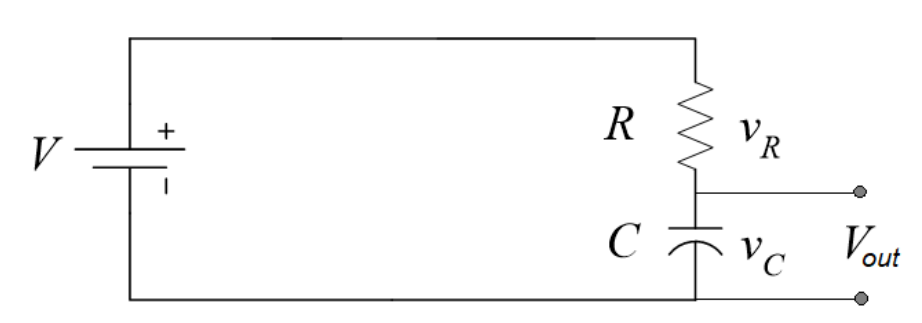
\includegraphics[scale = 0.55]{images/img1.png}
\label{filtro1}
\caption{Circuito RC - Exercício 01}
\end{figure}

\subsubsection{Entrada degrau [$V=A \>\ p/ \>\ t> 0$]}

Para uma entrada degrau com amplitude A, limitaremos a tensão de entrada a uma sugestão de $5V$, que será a tensão da fonte de alimentação que utilizaremos na simulação.\\

Assim, a equação para a tensão de saída será:

\begin{equation*}
    V(t) = A * ( 1 - e^{-t/0,1ms} ), \>\ para \>\ t > 0 \>\ e \>\ V(0) = 0
\end{equation*}

Que é o valor máximo da tensão de saída em um circuito RC após a carga completa do capacitor (derivada da equação de carga do capacitor).\\

A tensão de entrada será uma entrada degrau com amplitude $A = 5V$. \\

A simulação no LTSpice será feita usando o seguinte circuito:

\begin{figure}[H]
\centering
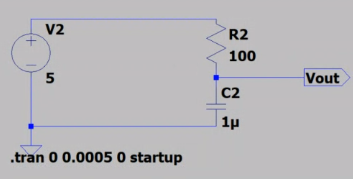
\includegraphics[scale = 0.75]{images/spice_1.png}
\label{filtro1}
\caption{Circuito 1.1.1 no LTSpice - Entrada degrau V=5V}
\end{figure}

A fonte de alimentação $V_1$ será configurada para fornecer a entrada degrau com amplitude de $5V$. O capacitor $C1$ e o resistor R1 formam o circuito $RC$. O resistor de carga $R_{load}$ é usado para medir a tensão de saída $V_{out}$.

Com o circuito e a equação de tensão de saída definidas, podemos proceder com a simulação. Executando a simulação no LTSpice, obtemos as seguintes formas de onda para as tensões no resistor, capacitor e saída:

\begin{figure}[H]
\centering
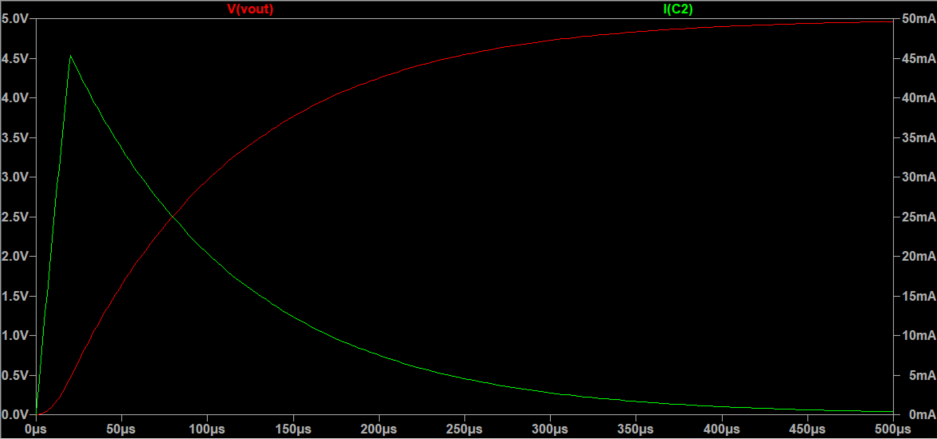
\includegraphics[scale = 0.65]{images/grafico_1_1.png}
\label{filtro1}
\caption{Gráfico da simulação 1.1.1 - Entrada degrau V=5V}
\end{figure}

Podemos ver que a tensão no capacitor começa em 0 e aumenta gradualmente até atingir cerca de 5.0V após $5\tau$ (0,5ms). A tensão de saída $V_{out}$ segue a mesma curva, mas com uma escala ajustada em relação à tensão de entrada. A constante de tempo do circuito é claramente visível novamente na forma de onda da tensão de saída, levando cerca de $5\tau$ para atingir o valor máximo de 4,9V.

Portanto, o circuito RC com $R = 100\Omega$ e $C = 1\mu F$ produz uma resposta suave à entrada degrau com amplitude $A = 5V$, com uma constante de tempo de $0,1ms$ e um valor máximo de tensão de saída de aproximadamente $5V$.


\subsubsection{Entrada senoidal $[V=V_0 cos(\omega t)]$ resposta p/ $t>>1$}
Para realizar a simulação do circuito RC com $R=100\Omega$ e $C=1\mu F$ com uma entrada senoidal de amplitude $V_0$ $cos(\omega t)$, fizemos o seguinte circuito esquemático no LTSpice, onde sugerimos uma tensão alternada de 5V:\\

\begin{figure}[H]
\centering
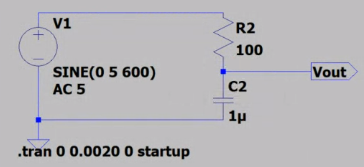
\includegraphics[scale = 0.75]{images/spice_2.png}
\label{filtro1}
\caption{Circuito 1.1.2 no LTSpice - Entrada senoidal}
\end{figure}

A resposta para $t >> 1/ \omega RC$ é a regime permanente, pois o circuito alcança um estado estável após um tempo suficientemente longo.

\begin{figure}[H]
\centering
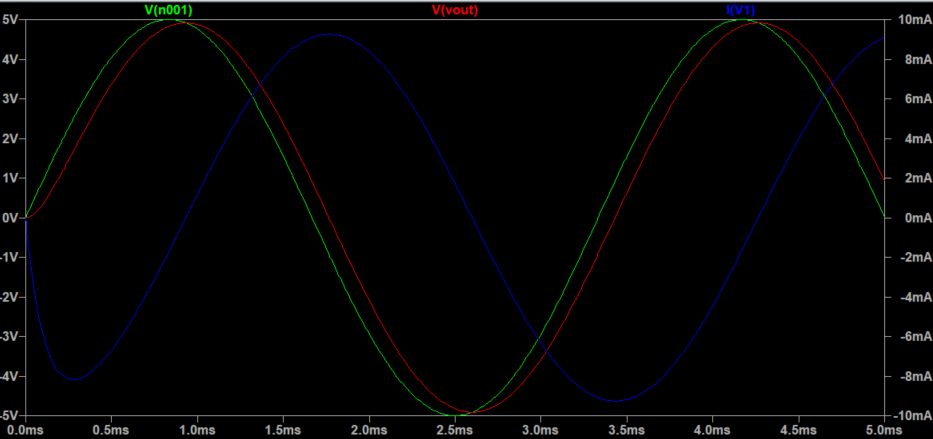
\includegraphics[scale = 0.65]{images/grafico_1_2.png}
\label{filtro1}
\caption{Gráfico da simulação 1.1.2 - Entrada senoidal}
\end{figure}



\subsubsection{Varredura de frequências [$\omega$ vs Ganho]}

\begin{figure}[H]
\centering
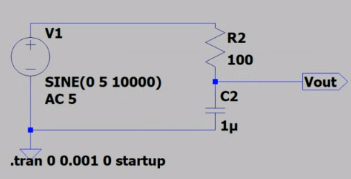
\includegraphics[scale = 0.75]{images/spice_3.png}
\label{filtro1}
\caption{Circuito 1.1.3 no LTSpice - Varredura de frequências}
\end{figure}


A resposta em frequência desse circuito pode ser dada pelo ganho em função da frequência de entrada, ou seja, a relação entre a amplitude do sinal de saída (Vout) e a amplitude do sinal de entrada (Vin). \\

Para este circuito, podemos calcular o ganho do filtro passa-baixas em função da frequência angular ($\omega$), utilizando a seguinte equação:\\

$$G(\omega) = \frac{V{out}}{V{in}} = \frac{1}{\sqrt{1+(\omega RC)^2}}$$\\

Substituindo os valores $R = 100\Omega$ e $C = 1 \mu F$, temos:\\

$$G(\omega) = \frac{1}{\sqrt{1+(\omega\times100\times10^{-6})^2}}$$\\

Podemos graficar a resposta desse circuito. Para isso, selecionamos um intervalo de frequências, representado em $\omega$. Para cada valor de $\omega$, calculamos o ganho correspondente. Assim, podemos plotar o ganho em função de $\omega$. \\

\begin{figure}[H]
\centering
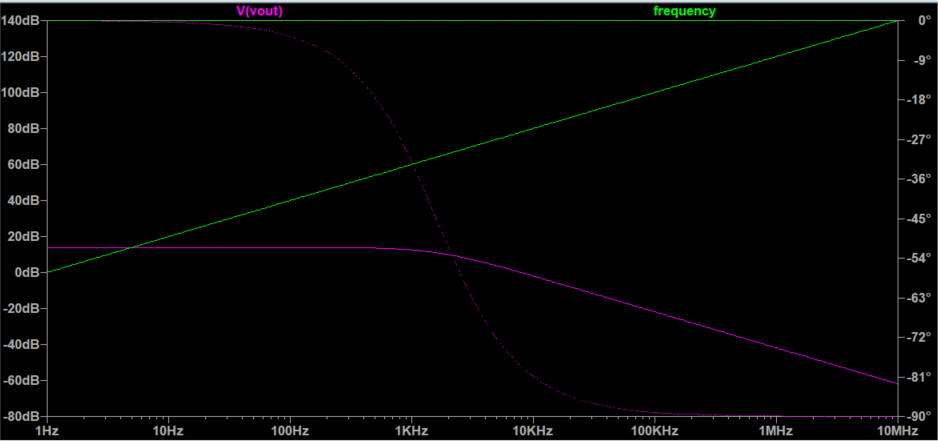
\includegraphics[scale = 0.65]{images/grafico_1_4.png}
\label{filtro1}
\caption{Gráfico 1 da simulação 1.1.3 - Varredura de frequências}
\end{figure}

O resultado é uma curva que gradualmente diminui à medida que a frequência aumenta. A curva se aproxima de 0 conforme a frequência se aproxima da frequência de corte ($f_c$, calculada anteriormente em cerca de $\omega_c=10^{-4}rad/s$). \\

Assim, uma varredura de frequências $\omega$ nesse circuito apresentará uma resposta de ganho em frequência que diminui conforme a frequência aumenta, com uma queda mais acentuada à medida que a frequência se aproxima de $\omega_c$.\\



\begin{figure}[H]
\centering
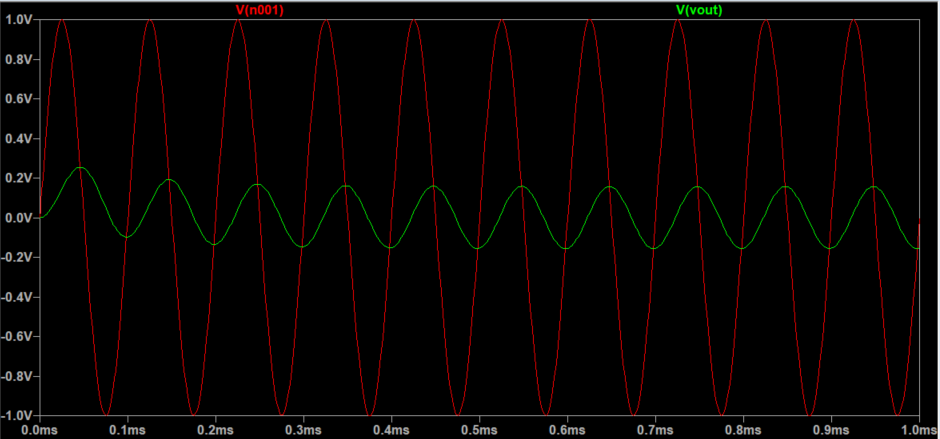
\includegraphics[scale = 0.65]{images/grafico_1_3.png}
\label{filtro1}
\caption{Gráfico 2 da simulação 1.1.3 - Filtragem}
\end{figure}



\newpage
\subsection{- Exercício}
\textbf{Fazer cálculo e simular circuito RC com
$R=100\Omega$, $C=1\mu F$.} \\

\begin{figure}[H]
\centering
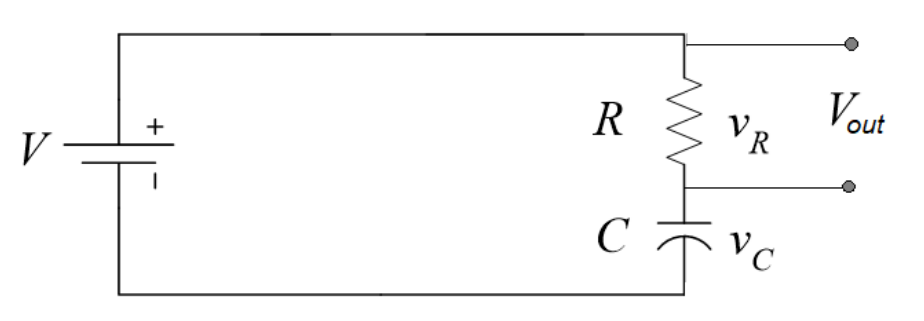
\includegraphics[scale = 0.55]{images/img2.png}
\label{filtro1}
\caption{Circuito RC - Exercício 02}
\end{figure}

\subsubsection{Entrada degrau [$V=A \>\ p/ \>\ t> 0$]}

Para calcular e simular o circuito, podemos fazer:\\

\textbf{a. Calcular a constante de tempo do circuito:\\
}
$\tau = R\cdot C = 100\Omega \cdot 1\mu F = 0,0001 s$\\

\textbf{b. Calcular a tensão no resistor VR e no capacitor VC:\\
}
Para t < 0, V = 0 V (condições iniciais)\\

Para t > 0, consideramos uma entrada degrau com V = A\\

A tensão no resistor VR pode ser calculada pela Lei de Ohm:\\

$VR = V\cdot \dfrac{R}{R+1/\omega C} = A \cdot \dfrac{100}{100+1/(0,0001\cdot \pi)} = A \cdot 0,9996$\\

A tensão no capacitor VC pode ser calculada usando a equação de carga de um capacitor:\\

$VC = V_{max} \cdot (1-e^{-t/\tau}) = A \cdot (1-e^{-t/(0,0001)})$\\

\textbf{c. Calcular a tensão de saída Vout:
}\\

A tensão de saída é igual à tensão no capacitor:\\

$Vout = VC = A \cdot (1-e^{-t/(0,0001)})$\\

\begin{figure}[H]
\centering
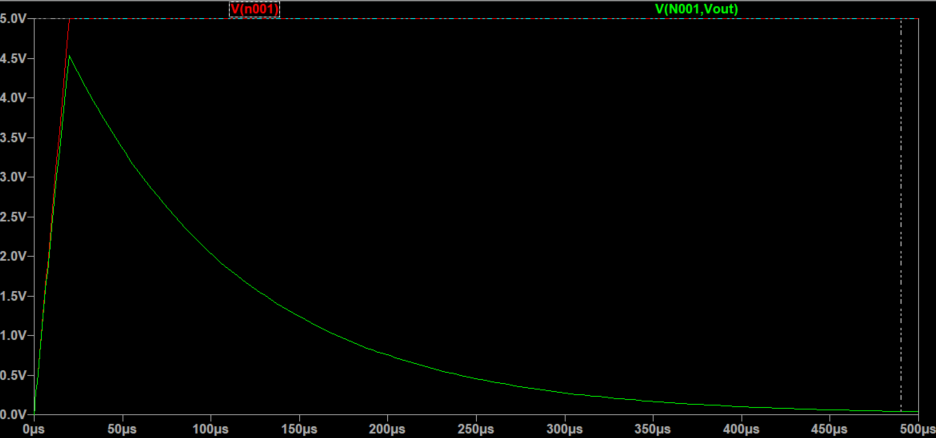
\includegraphics[scale = 0.65]{images/grafico_2_1.png}
\label{filtro1}
\caption{Gráfico da simulação 1.2.1 no LTSpice - Entrada degrau}
\end{figure}


\subsubsection{Entrada senoidal $[V=V_0 cos(\omega t)]$ resposta p/ $t>>1$}

a. Calcular a impedância do capacitor:

$ZC = \frac{1}{j \omega C} = \frac{-j}{\omega C} = -j10^3 \Omega,$ onde $\omega = 2\pi f$ é a frequência angular da entrada e $f$ é a frequência em Hertz.

b. Calcular a impedância total do circuito:

$Z{total} = R + Z_C = R - j10^3 \Omega$

c. Calcular a amplitude da corrente do circuito:

$i = \frac{V0}{|Z{total}|}=\frac{V_0}{\sqrt{R^2 + 10^6 \Omega^2}}$

d. Calcular a fase da corrente em relação à tensão de entrada:

$\theta = \arctan \left( \frac{-10^3 \Omega}{R} \right)$

e. Calcular a amplitude da tensão no resistor VR:

$VR = i \cdot R = \frac{V_0 \cdot R}{\sqrt{R^2 + 10^6 \Omega^2}}$

f. Calcular a amplitude da tensão no capacitor VC:

$VC = V_0 \cdot |Z_C| \cdot \frac{1}{\sqrt{R^2 + 10^6 \Omega^2}} = V0 \cdot \frac{1}{\sqrt{R^2 + 10^6 \Omega^2}} \cdot 10^3 \Omega$

g. Calcular a amplitude da tensão de saída Vout:

$V{out} = VC$

h. Calcular a fase da tensão de saída em relação à tensão de entrada:

$\phi = -\frac{\pi}{2}$ (devido à fase de $ZC$ ser de $-90^\circ$)

Dessa forma, a resposta do circuito RC para $t>>1$ é uma senoide com amplitude $V{out} = V_0 \cdot \frac{1}{\sqrt{R^2 + 10^6 \Omega^2}} \cdot 10^3 \Omega$ e fase $-\frac{\pi}{2}$ em relação à entrada.


\begin{figure}[H]
\centering
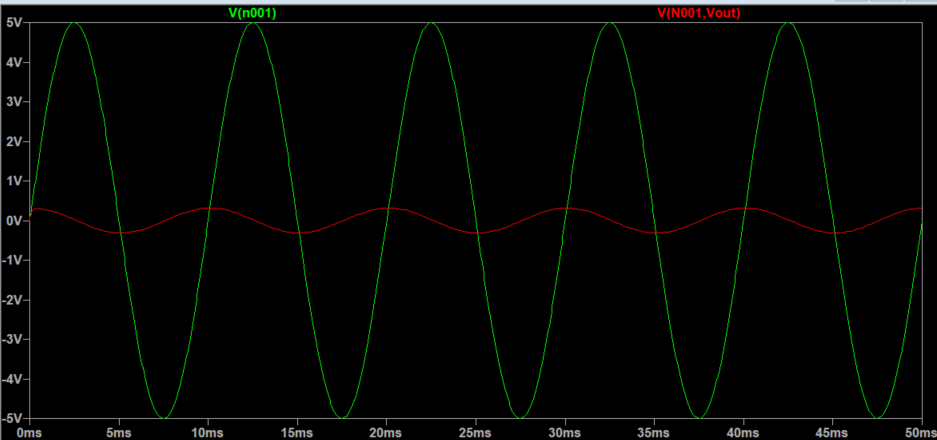
\includegraphics[scale = 0.65]{images/grafico_2_2.png}
\label{filtro1}
\caption{Gráfico da simulação 1.2.2 no LTSpice - Entrada Senoidal}
\end{figure}


\subsubsection{Varredura de frequências [$\omega$ vs Ganho]}

\begin{figure}[H]
\centering
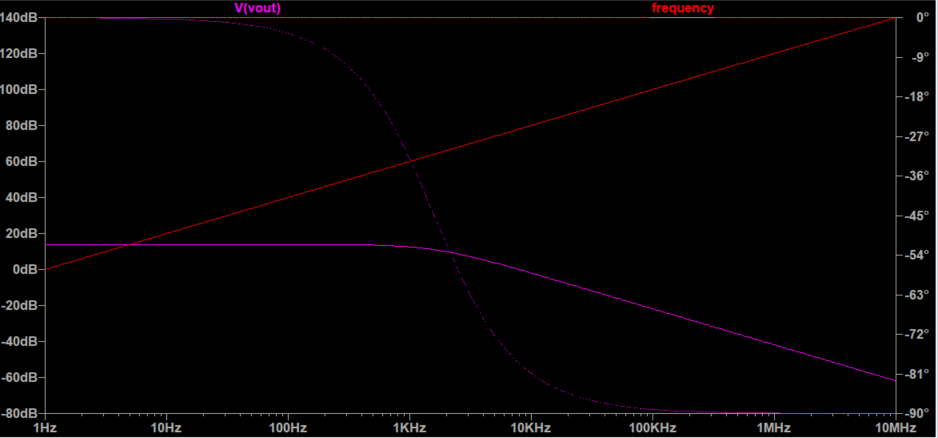
\includegraphics[scale = 0.65]{images/grafico_2_4.png}
\label{filtro1}
\caption{Gráfico 1 da simulação 1.2.3 no LTSpice - Varredura de frequências}
\end{figure}

\begin{figure}[H]
\centering
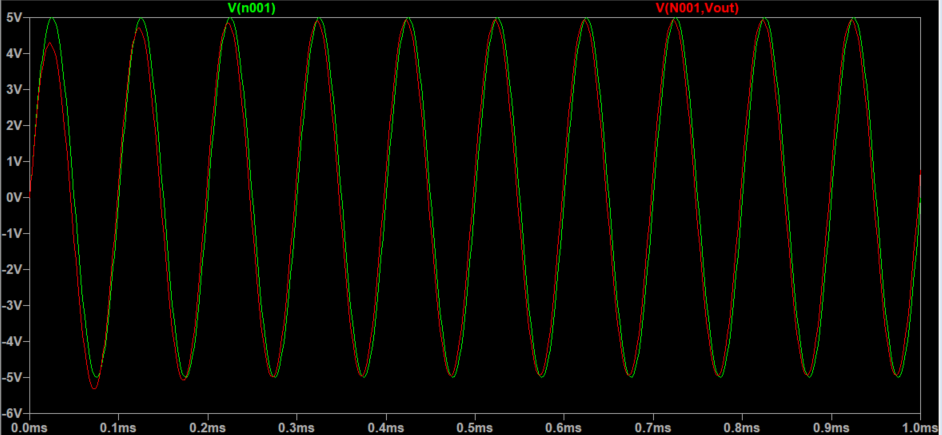
\includegraphics[scale = 0.65]{images/grafico_2_3.png}
\label{filtro1}
\caption{Gráfico 2 da simulação 1.2.3 no LTSpice - filtragem}
\end{figure}



\newpage
\subsection{- Exercício}
\textbf{Fazer cálculo e simular circuito RL com
$R=100\Omega$, $L=1 H F$.} \\
\begin{figure}[H]
\centering
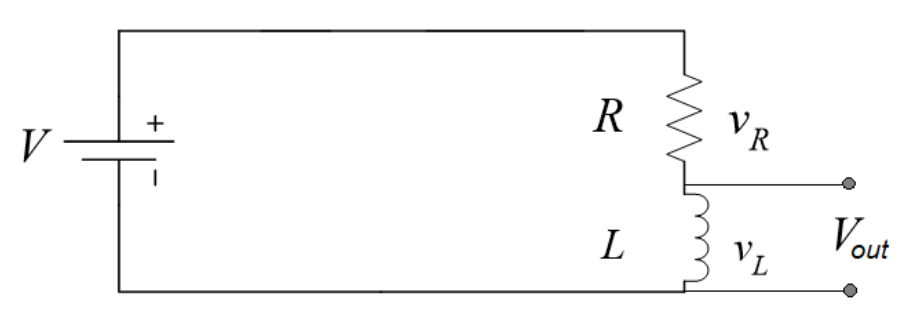
\includegraphics[scale = 0.55]{images/img3.png}
\label{filtro1}
\caption{Circuito RL - Exercício 03}
\end{figure}

\subsubsection{Entrada degrau [$V=A \>\ p/ \>\ t> 0$]}

\begin{figure}[H]
\centering
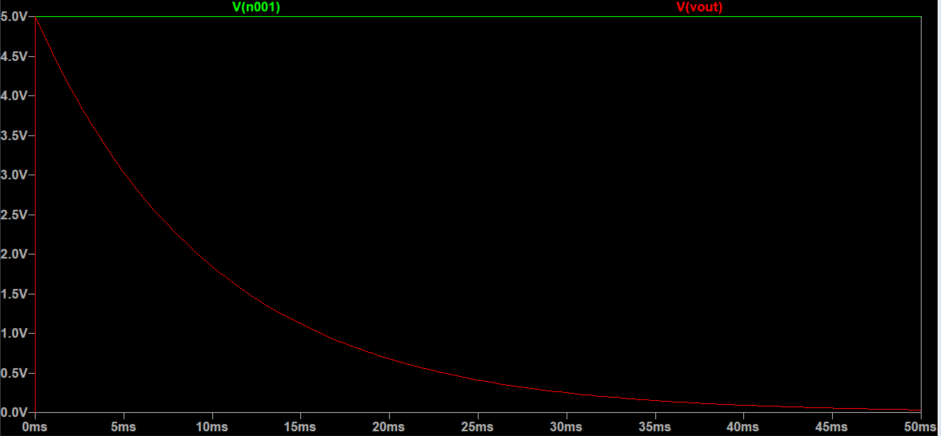
\includegraphics[scale = 0.65]{images/grafico_3_1.png}
\label{filtro1}
\caption{Gráfico da simulação 1.3.1 no LTSpice - Entrada degrau }
\end{figure}

\subsubsection{Entrada senoidal $[V=-V_0 sen(\omega t)]$ resposta p/ $t>>1$}

\begin{figure}[H]
\centering
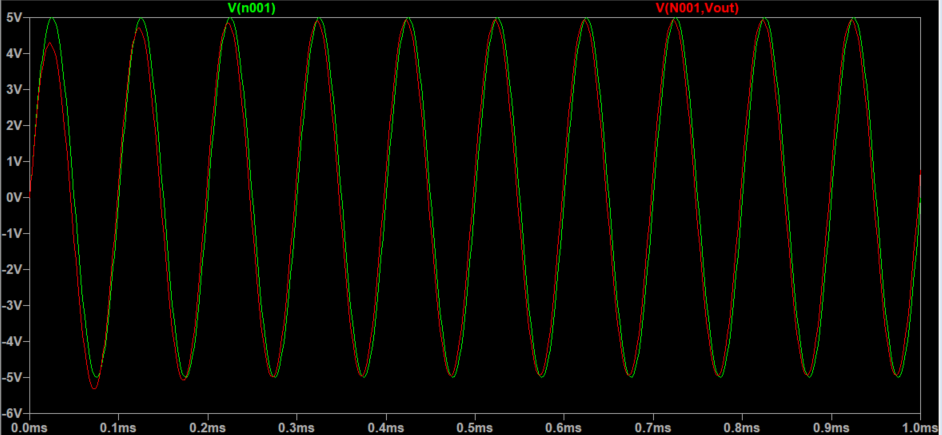
\includegraphics[scale = 0.45]{images/grafico_3_2.png}
\label{filtro1}
\caption{Gráfico da simulação 1.3.2 no LTSpice - Entrada senoidal }
\end{figure}



\subsubsection{Varredura de frequências [$\omega$ vs Ganho]}

\begin{figure}[H]
\centering
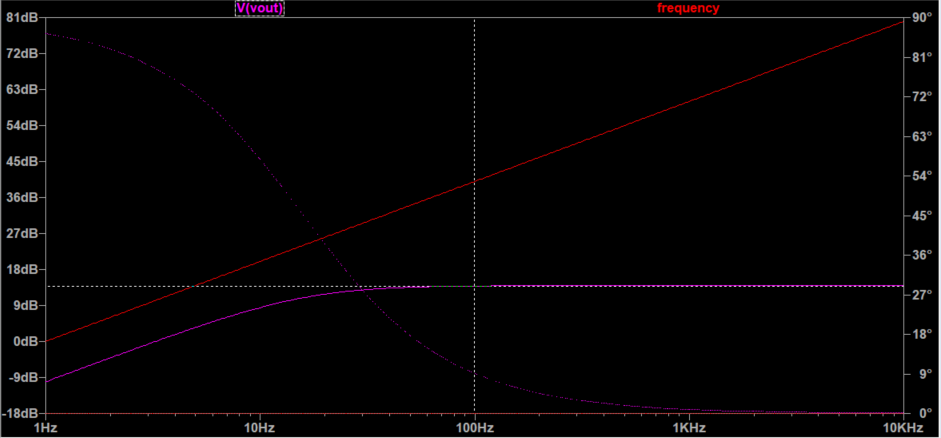
\includegraphics[scale = 0.65]{images/grafico_3_3.png}
\label{filtro1}
\caption{Gráfico da simulação 1.3.3 no LTSpice - Varredura de frequências}
\end{figure}
















\newpage
\subsection{- Exercício}
\textbf{Fazer cálculo e simular circuito RLC com
$R=100\Omega$, $C = 1\mu F$, $L=1 H F$.} \\
\begin{figure}[H]
\centering
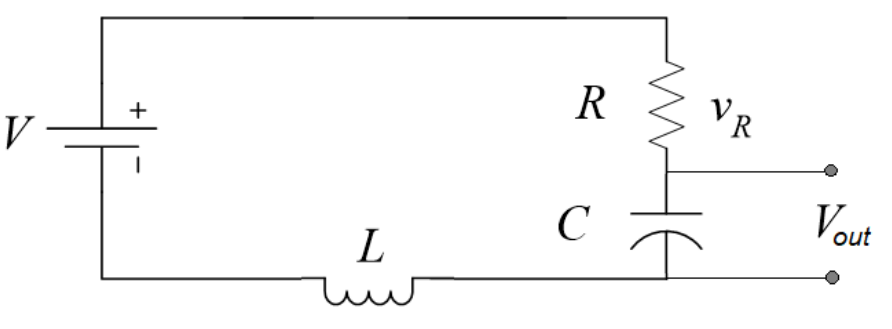
\includegraphics[scale = 0.55]{images/img4.png}
\label{filtro1}
\caption{Circuito RLC - Exercício 04}
\end{figure}

\subsubsection{Entrada degrau [$V=A \>\ p/ \>\ t> 0$]}

Para uma entrada degrau com amplitude A, limitaremos a tensão de entrada a uma sugestão de $5V$, que será a tensão da fonte de alimentação que utilizaremos na simulação.\\

Assim, a equação para a tensão de saída será:

\begin{equation*}
    v(t) = e^{-\zeta \omega_n t} (A \cos(\omega_d t) + B \sin(\omega_d t))
\end{equation*}

Que é o valor máximo da tensão de saída em um circuito RLC série após a carga completa do capacitor e a corrente no indutor.\\

A tensão de entrada será uma entrada degrau com amplitude $A = 5V$. \\

A simulação no LTSpice será feita usando o seguinte circuito:

\begin{figure}[H]
\centering
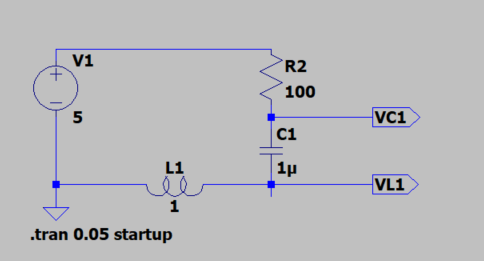
\includegraphics[scale = 0.75]{images/spice_4_1.png}
\label{filtro1}
\caption{Circuito 1.4.1 no LTSpice - Entrada degrau}
\end{figure}



\begin{figure}[H]
\centering
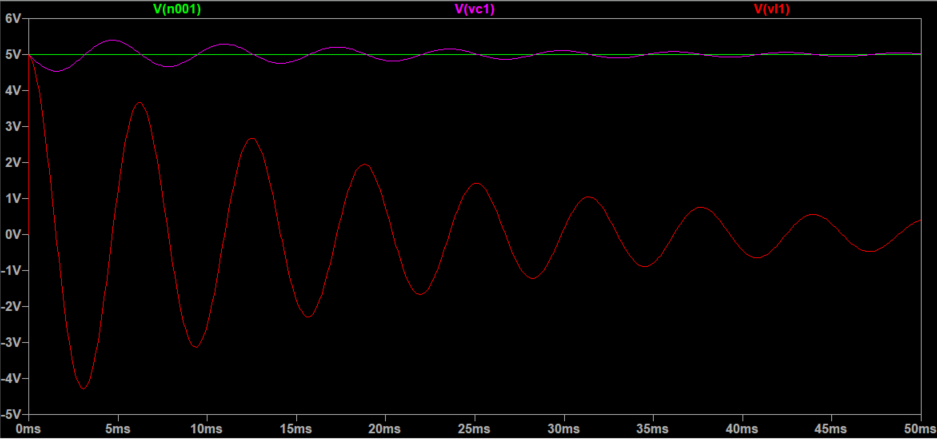
\includegraphics[scale = 0.65]{images/grafico_4_1.png}
\label{filtro1}
\caption{Gráfico da simulação 1.4.1 no LTSpice - Entrada degrau}
\end{figure}


\subsubsection{Entrada senoidal $[V=-V_0 sen(\omega t)]$ resposta p/ $t>>1$}


Para realizar a simulação do circuito RC com $R=100\Omega$ , $L=1 H F$ e $C=1\mu F$ com uma entrada senoidal de amplitude $V_0$ $cos(\omega t)$, fizemos o seguinte circuito esquemático no LTSpice, onde sugerimos uma tensão alternada de 5V:\\

\begin{figure}[H]
\centering
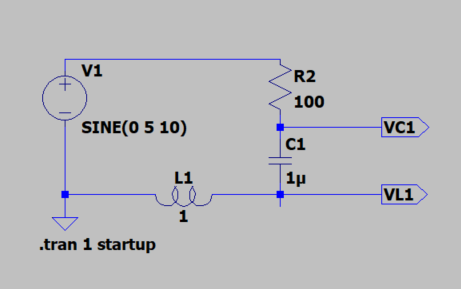
\includegraphics[scale = 0.75]{images/spice_4_2.png}
\label{filtro1}
\caption{Circuito 1.4.2 no LTSpice - Entrada senoidal}
\end{figure}

A resposta para $t >> 1/ \omega RLC$ é a regime permanente, pois o circuito alcança um estado estável após um tempo suficientemente longo.

\begin{figure}[H]
\centering
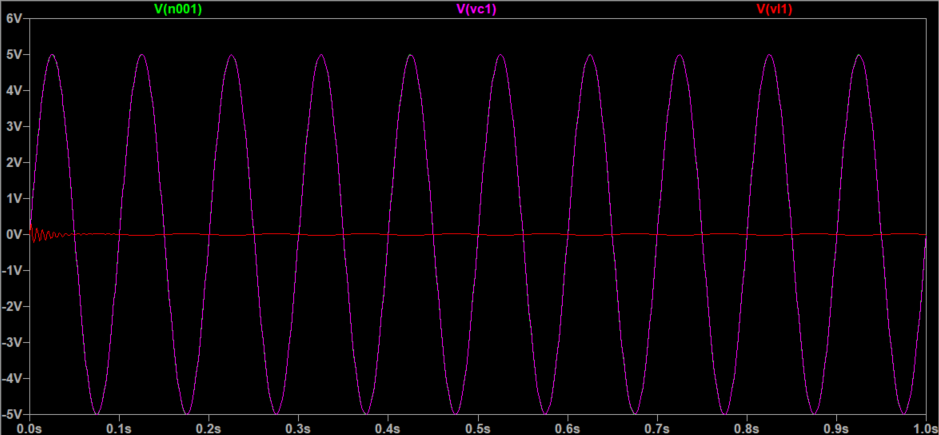
\includegraphics[scale = 0.65]{images/grafico_4_2.png}
\label{filtro1}
\caption{Gráfico da simulação 1.4.2 no LTSpice - Entrada senoidal}
\end{figure}


\subsubsection{Varredura de frequências [$\omega$ vs Ganho]}
\begin{figure}[H]
\centering
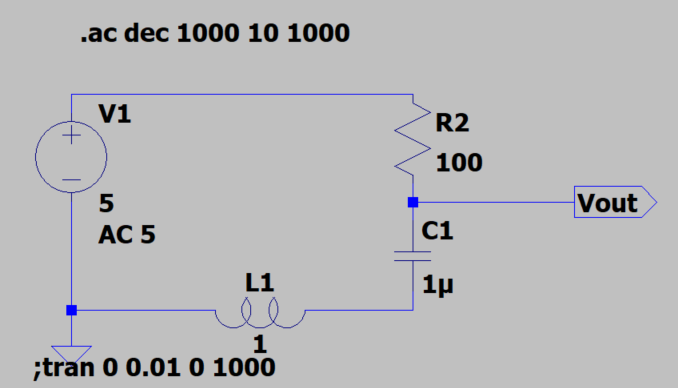
\includegraphics[scale = 0.75]{images/spice_4_3.png}
\label{filtro1}
\caption{Circuito 1.4.3 no LTSpice - Varredura de frequências}
\end{figure}

A resposta em frequência desse circuito pode ser dada pelo ganho em função da frequência de entrada, ou seja, a relação entre a amplitude do sinal de saída (Vout) e a amplitude do sinal de entrada (Vin). \\

Para este circuito, podemos calcular o ganho do filtro passa-faixa em função da frequência angular ($\omega$), utilizando a seguinte equação:\\

$$G(\omega) = \frac{\omega RC}{\sqrt{(\omega^2-\omega_0^2)^2 + (\frac{\omega \omega_0 R}{L})^2}}
$$\\

Substituindo os valores $R = 100\Omega$ ,$L=1 H F$ e $C = 1 \mu F$, temos:\\

$$G(\omega) = \frac{\omega (100\text{Ω})(1\text{μF})}{\sqrt{(\omega^2-(10^5)^2)^2 + (\frac{\omega (10^5)(100\text{Ω})}{(1\text{H})})^2}}

$$\\

Podemos graficar a resposta desse circuito. Para isso, selecionamos um intervalo de frequências, representado em $\omega$. Para cada valor de $\omega$, calculamos o ganho correspondente. Assim, podemos plotar o ganho em função de $\omega$. \\

\begin{figure}[H]
\centering
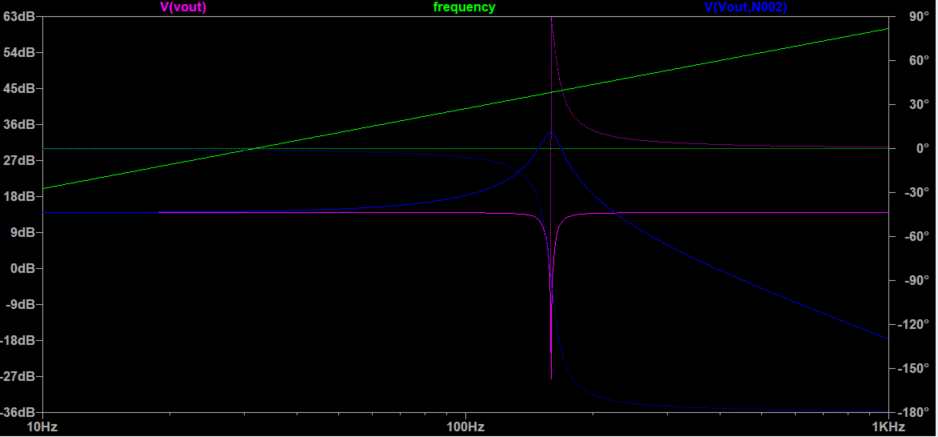
\includegraphics[scale = 0.65]{images/grafico_4_3.png}
\label{filtro1}
\caption{Gráfico da simulação 1.4.3 no LTSpice - Varredura de frequências}
\end{figure}

\newpage
% REFERENCIAS %%%%%%%%%%%%%%%%%%%%%%%%%%%%%%%%%%%%%%%%%%%%%%%%%%%%%%%%%%%%%%


\end{document}